\documentclass[runningheads]{llncs}
%
\usepackage[T1]{fontenc}
% T1 fonts will be used to generate the final print and online PDFs,
% so please use T1 fonts in your manuscript whenever possible.
% Other font encondings may result in incorrect characters.
%
\usepackage{graphicx}
\usepackage{float}
\usepackage{comment}
% Used for displaying figures. If possible, figure files should
% be included in EPS format.
%
% If you use the hyperref package, please uncomment the following two lines
% to display URLs in blue roman font according to Springer's eBook style:
%\usepackage{color}
%\renewcommand\UrlFont{\color{blue}\rmfamily}
\usepackage{hyperref}
\urlstyle{rm}
%
\begin{document}
%
\title{A Layered Architecture for Digital Twins with Progressive Fidelity: A Case Study in Airport Operations with Specification-First Development}
%
\titlerunning{Digital Twins for Progressive Fidelity}
%
\author{Arthur Chevallier \and German Castignani}
%
\authorrunning{A. Chevallier and G. Castignani}
%
\institute{Luxembourg Institute of Science and Technology\\
\email{arthur.chevallier@list.lu, german.castignani@list.lu}}
%
\maketitle % typeset the header of the contribution
%
\begin{abstract}
Digital twins of complex cyber-physical systems rarely start at full resolution: they must grow incrementally from simple representations towards higher fidelity, in terms of spatial granularity, temporal resolution, and behavioural realism, by integrating physical layouts, geospatial and live data, and decision support. Existing digital-twin architectures decompose a twin into layers, but do not explicitly address how fidelity can be increased without restructuring what is already implemented. We propose a four-layer architecture in which each layer exposes an explicit contract to the layer above, so that raising the fidelity of one layer extends, rather than rewrites, the layers around it. The topmost layer is decisional and hosts the twin's analytical and machine-learning capabilities, with actions reaching the source system only through approval gates. To keep implementations aligned with these contracts, we adopt a specification-first methodology in which event schemas, data models, and per-service specifications are written first and remain authoritative. We instantiate the architecture in VirtualSky International Airport (EVSK), a fully open-source airport digital twin of nine microservices covering flight operations, passenger flows, baggage handling, weather, incident cascades, cost analysis, and planning. An audit of EVSK's change history examines whether capabilities were added by extending existing contracts, and a mid-project audit identifies where specifications alone did not guarantee conformance. The results support explicit inter-layer contracts, backed by systematic verification, as a practical principle for evolving digital twins.

\keywords{Digital twins \and Progressive fidelity \and Layered architecture \and Airport operations \and Specification-driven development \and Decision support.}
\end{abstract}
%
%
%
\section{Introduction}\label{sec:introduction}

Digital twins are virtual counterparts of physical systems maintained through structured data flows~\cite{glaessgen2012,grieves2017}. In complex domains such as aviation, they cannot be built at maximum resolution from the outset: data, models, and integrations become available incrementally. A project may begin with a logical event model and later add physical simulation, geospatial representation, live data, analytics, and decision support. Throughout this paper, \emph{fidelity} denotes how closely a twin matches its physical counterpart along spatial, temporal, and behavioural dimensions (Section~\ref{sec:architecture}), thereby supporting more reliable feedback and decision making. Increasing any dimension can alter representations, interfaces, and data flows already used by earlier capabilities. Extension can therefore become restructuring, hindering long-term evolution and reproducibility~\cite{jones2020}.

Existing frameworks provide important decompositions. ISO 23247 defines a manufacturing reference architecture~\cite{iso23247}, Tao et al.\ separate the physical entity, virtual entity, data, services, and connections~\cite{tao2018}, and Redelinghuys et al.\ separate concerns from acquisition to emulation~\cite{redelinghuys2019}. They do not explicitly make \emph{fidelity-preserving evolution} a constraint: higher-fidelity capabilities should extend the contracts of lower layers rather than restructure them. This is the gap investigated here.

We therefore ask:

\begin{quote}
\textbf{RQ1: How can a digital-twin architecture support progressive increases in fidelity while preserving the contracts and functionality of previously implemented layers?}
\end{quote}

We study EVSK, the VirtualSky International Airport digital twin and an ongoing research prototype. Its operational entities and ground truth are synthetic, except for opt-in L2 live ADS-B and METAR feeds. Airports provide a demanding testbed because aircraft, vehicles, passengers, baggage, infrastructure, schedules, weather, and disruptions interact across multiple operational timescales. Existing research provides mature models for individual aspects of this system, including delay propagation~\cite{pyrgiotis2013}, delay cost~\cite{cook2009}, passenger-flow prediction~\cite{ke2017,schultz2019}, and airport digital twins~\cite{conde2024,palasca2025}. EVSK instead uses the airport as an instrument for studying whether progressively richer representations can share stable contracts. Its implementation comprises nine FastAPI domain services behind one API gateway, including a decisional layer for anomaly detection, scenario analysis, optimisation, appraisal, and gated recommendations.

The second question concerns how such an architecture can be implemented and maintained without its contracts eroding. Event schemas, shared concepts, service boundaries, and data flows must remain coherent as a distributed system evolves, and the local correctness of individual changes does not guarantee this. We therefore use a specification-first methodology in which service specifications, event schemas, data models, and simulation rules are defined before implementation and remain authoritative, supplemented by reusable ``skill files'' encoding implementation patterns and known pitfalls. Implementation was assisted by coding agents; we treat this as operational context, and Section~\ref{sec:methodology} delimits where human intervention was required. This motivates:

\begin{quote}
\textbf{RQ2: To what extent does specification-first development preserve architectural contracts during sustained implementation of a progressively evolving digital twin, and where does it require independent verification?}
\end{quote}

The paper makes four contributions:
\begin{enumerate}
\item a layered fidelity architecture that treats progressive, contract-preserving evolution as an explicit architectural principle, with fidelity defined along spatial, temporal, and behavioural dimensions;
\item a specification-first development methodology for maintaining these architectural contracts during implementation;
\item EVSK, a fully open-source airport digital-twin prototype that instantiates the architecture across four layers, including established analytical and ML components used to exercise the layer boundaries; and
\item an empirical examination of the principle, combining an analysis of how changes propagated across layers with an audit of where implementation departed from specification.
\end{enumerate}

The research object is therefore not the act of implementing an airport application, nor a new machine-learning method. It is the architectural principle and its empirical examination; EVSK is the single-case instrument through which contract preservation and violations are observed. The methodology is the engineering discipline used to maintain the principle, together with evidence of where specifications alone were not sufficient.

The remainder of the paper is organised as follows. Section~\ref{sec:related} discusses related work. Section~\ref{sec:architecture} presents the layered fidelity architecture, Section~\ref{sec:methodology} describes the development methodology, and Section~\ref{sec:implementation} presents EVSK. Section~\ref{sec:evaluation} reports the evaluation, followed by discussion and conclusions in Section~\ref{sec:discussion}.


\section{Related Work}\label{sec:related}

Digital-twin research provides several foundations for the architecture considered here. The concept originated as a virtual counterpart of a physical system~\cite{grieves2017} and was subsequently formalised as a lifecycle-spanning computational representation~\cite{glaessgen2012}. Kritzinger et al.~\cite{kritzinger2018} distinguish digital models, digital shadows, and digital twins according to the degree and direction of automated data exchange. Reference architectures such as ISO 23247~\cite{iso23247}, RAMI 4.0~\cite{rami40}, and the architecture proposed by Redelinghuys et al.~\cite{redelinghuys2019} provide different forms of decomposition into entities, layers, and services. Reviews nevertheless identify extensibility, interoperability, and reproducibility as continuing challenges~\cite{jones2020,mohammadi2017}. Our work addresses a narrower question within this literature: how to make increasing fidelity an explicit, contract-preserving evolution mechanism rather than simply a collection of architectural layers.

Airport modelling provides the application context for examining this question. Analytical and simulation-based research has addressed delay propagation~\cite{pyrgiotis2013} and the cost of delay~\cite{cook2009}, while machine learning has been applied to passenger-flow and boarding-time prediction~\cite{ke2017,schultz2019}. More recent work explicitly applies digital-twin concepts to airport operations, including turnaround operations~\cite{conde2024}, landside simulation~\cite{palasca2025}, and airport-wide adoption guidance~\cite{acrp2024}. These studies demonstrate the feasibility and value of airport digital twins, but generally address particular operational scopes or fixed capabilities rather than the problem of evolving a twin across fidelity levels without restructuring previously implemented functionality. EVSK uses the domain as a demanding instantiation of the architectural principle rather than as the primary research contribution.

Finally, AI-assisted software engineering has progressed from code synthesis~\cite{chen2021codex} and controlled productivity studies~\cite{peng2023copilot} to repository-level benchmarks such as SWE-bench~\cite{swebench2024} and agent-based development environments~\cite{yang2024sweagent}. Approaches such as MetaGPT further demonstrate the value of explicit software-development procedures for coordinating agents~\cite{hong2024metagpt}. These studies primarily evaluate local task completion or repository-level issue resolution. They provide less evidence about maintaining architectural consistency across a long-running, distributed system as new capabilities are added. Our work investigates whether specification-first development can provide such a constraint, using the progressive-fidelity architecture as the concrete setting.

The resulting gap is therefore the combination of two problems: \emph{how to evolve a digital twin across fidelity levels without restructuring existing layers, and how to maintain the resulting architectural contracts during sustained agent-assisted development}. RQ1 addresses the architectural problem. RQ2 addresses the engineering process used to implement it.

\section{Layered Fidelity Architecture}\label{sec:architecture}

\subsection{Fidelity and why it must be progressive}

We define the \emph{fidelity} of a digital twin along three dimensions: \emph{spatial granularity}, from topological relations between entities to gate-level coordinates and geometry; \emph{temporal resolution}, from discrete simulated events to sub-second live updates; and \emph{behavioural realism}, from discrete state transitions to physically grounded and data-calibrated dynamics. In complex domains such as aviation, a twin cannot be built at maximum resolution from the outset. The required data, models, and integrations become available over time, and each must be added to a system that already works. Fidelity is therefore acquired progressively, and the architectural question is whether each increase can be made without restructuring what is already implemented.

\subsection{Four capability layers}

The architecture is a stack of four capability layers, each of which raises fidelity along a different combination of the three dimensions (Table~\ref{tab:fidelity}):

\begin{itemize}
\item \textbf{L0, logical event-driven simulation.} Domain entities are represented as state machines that communicate purely through events. There is no geometry and no external data at this layer. Something happens, an event records it, and downstream consumers react.
\item \textbf{L1, physical layer.} Spatial layout is added on top of L0: positions, distances, and the travel or transfer times they induce between entities already defined at L0.
\item \textbf{L2, geospatial and real-world data layer.} The twin is connected to the outside world. Map-based visualisation, live external feeds, and reference data ground the logical and physical state in observed reality.
\item \textbf{L3, decisional layer.} Forecasting, scenario analysis, anomaly detection, optimisation, and recommendation are built on the first three layers. Actions reach the source system only through approval gates.
\end{itemize}

\begin{table}[H]
\centering
\caption{Fidelity gained at each layer, with the corresponding EVSK capability.}
\label{tab:fidelity}
\begin{tabular}{llll}
\hline
Layer & Spatial & Temporal & Behavioural \\
\hline
L0 & topological & discrete events & state transitions \\
L1 & gate-level geometry & unchanged & travel and transfer times \\
L2 & georeferenced & live and historical feeds & data-calibrated \\
L3 & --- & forecast horizons & prescriptive, gated actions \\
\hline
\end{tabular}
\end{table}

Figure~\ref{fig:architecture} summarises this domain-independent stack and shows how its four layers map to the EVSK airport implementation.

\begin{figure}[H]
\centering
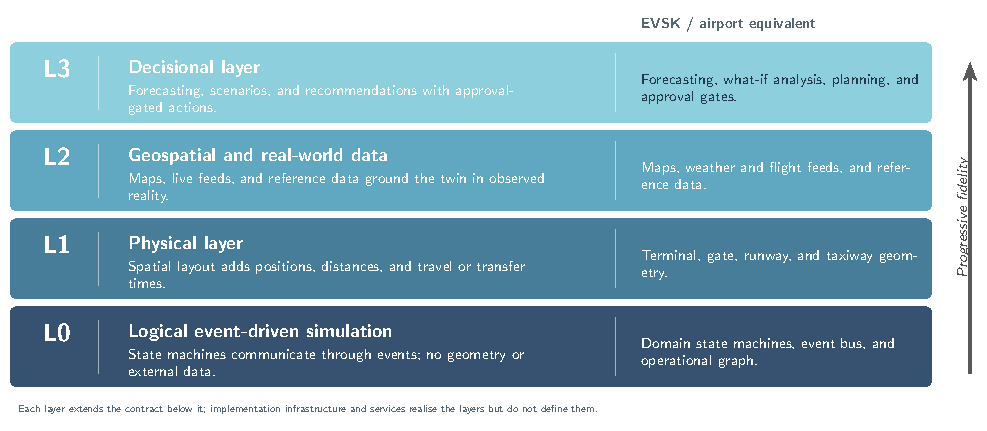
\includegraphics[width=\textwidth]{figures/arch.pdf}
\caption{Generalized four-layer architecture for progressive fidelity, with the corresponding EVSK airport capabilities shown at right. Each layer extends the contract exposed by the layer below it.}
\label{fig:architecture}
\end{figure}

L0 to L2 form a digital shadow: data flows from the physical system, or from its simulated stand-in, into the twin~\cite{kritzinger2018}. L3 closes the loop by acting as the command gate through which decisions return to the source system.

A separate axis governs how a single layer matures, independent of which layer it is. Capability within a layer deepens along a fixed ladder, from visualisation, to monitoring and alerting, to prediction, to prescription, to actionability. This ladder describes what a layer \emph{does}, whereas fidelity describes how closely it \emph{represents}; a layer counts as mature once it has climbed the ladder, not merely because it renders something.

\subsection{Contracts and the fidelity-preservation invariant}

Each layer $L_i$ exposes a contract $C_i$ to the layers above it: the event schemas it publishes, the graph model it owns, and the service interfaces it offers. Two rules govern dependencies. A layer may depend on the contracts of lower layers but never on the internals of any layer, and nothing below a layer ever depends on it. In particular, L3 may read from L0--L2, but nothing below L3 imports from it, which keeps the decisional layer removable without destabilising the shadow underneath.

These rules yield the architectural invariant on which the rest of the paper rests:

\begin{quote}
\textbf{Fidelity-preservation invariant.} Raising the fidelity of layer $L_i$ may extend its contract $C_i$, but must not modify or remove any existing element of any contract $C_j$. Consequently, layers above $L_i$ continue to operate unchanged.
\end{quote}

For example, replacing synthetic weather with a live METAR feed changes the implementation of an L2 adapter, but the events that L3 consumes keep the same schema. Upgrading a layer's fidelity thus changes that layer's modules and, at most, adds to its contract, and it does not trigger refactoring in the layers that consume it. Section~\ref{sec:evaluation} tests this property against the development history of EVSK.

\subsection{The L2 to L3 boundary}

Because L3 can trigger actions, corrupted data crossing from L2 into the decisional layer is the most consequential failure. The boundary is therefore defined at the contract level rather than left to each analytical component. Every source, whether simulated, historical, or live, is normalised by an adapter into the same domain events (Section~\ref{sec:implementation}), so validation is applied once, at the adapter, and not re-implemented in each consumer.
% TODO(Arthur): state the checks actually implemented, e.g. schema validation of event envelopes, range/plausibility checks on METAR and ADS-B inputs, outlier or duplicate filtering, idempotency handling. If some are not implemented, say so and move them to future work.
Decisions derived from this data do not act directly. Recommendations enter an approval queue and are classified as auto-executable, human-gated, safety-guarded, or operator-blocked, and reach other domains only through per-domain command topics.

\subsection{Generality}

What the architecture fixes is the order in which fidelity is added and the contracts between layers, not the domain those layers describe. A hospital campus twin could follow the same order: patient, staff, and equipment state machines on an event bus at the base, ward and building layout above, real-time location and environmental sensing next, and bed-allocation or staffing optimisation at the top. The same layering applies to smart ports, manufacturing plants, and urban mobility networks. We use an airport, EVSK, as the concrete instantiation and stress test in the remainder of the paper.

Section~\ref{sec:implementation} shows how EVSK realises each layer with a concrete technology stack, together with the architectural invariants that keep them composable in practice.

\section{Enforcing Layer Contracts with Specification-First Development}\label{sec:methodology}

The layered architecture in Section~\ref{sec:architecture} keeps fidelity additions from forcing a rewrite by fixing what each layer may depend on. That guarantee holds only if the implementation actually respects those contracts, and nothing about the architecture enforces that on its own. The methodology that keeps the two aligned rests on an inversion of the usual workflow: the specification is written first, is machine-readable, and is authoritative. Implementation may not deviate from it, and where reality demands a change, the spec is updated first and the code follows. Before any service is implemented, four definitions already exist: the event-bus schemas, the graph data model, the simulation rules, and one specification per service describing its endpoints, events, state machines, and ownership boundaries. Each new layer, in practice, starts as a specification of the contract it will expose to the layer above and consume from the layer below, before a single line of that layer's code is written.

This discipline has an intellectual lineage older than coding assistants. Writing the authoritative description before the implementation echoes formal specification traditions~\cite{lamport2002}, and decomposing the system so that each service hides exactly one set of design decisions follows Parnas' information-hiding criteria~\cite{parnas1972}. Because the specifications are machine-readable, they can also serve as the context for automated coding assistance, which made drift between specification and code more costly than in a purely manual workflow.

Complementing the per-service and per-layer specifications are ``skill files'', which encode reusable project knowledge in a form readable by both humans and coding assistants. Each skill file has three parts: concept explanation, copy-paste patterns, and gotchas. The patterns keep new code consistent with the project's idioms, and the gotchas encode failures that review caught the hard way, so the same mistake is not repeated. Cross-cutting skills exist for exactly the four runtime invariants of EVSK (Section~\ref{sec:implementation}): the simulation clock, the event bus, the graph as single source of truth, and the no-silent-mutation rule. These are the invariants most likely to be violated under time pressure, since violating any one of them is often the fastest way to make a feature appear to work. Each service additionally owns one skill file documenting its own state machines and quirks.

Entry-point files (\texttt{CLAUDE.md}, \texttt{AGENTS.md}, and editor rule files) instruct the assistant to load the relevant specification and skill file before writing code. Hard rules act as guardrails, and each one maps directly onto a layer contract rather than a general best practice: no wall-clock time in business logic, no service-to-service HTTP calls, no silent mutations, and all data synthetic. Because each rule corresponds to a specific invariant, a violation is detectable by search or contract test, rather than surfacing later as a layer-boundary failure that looks unrelated to its cause.

\paragraph{Role of coding assistants and the human perimeter.}
EVSK was implemented with the help of AI coding assistants operating inside this specification framework. We treat this as operational context and not as a contribution, and we delimit it precisely. The assistants produced code within the boundaries set by the specifications. Humans were responsible for everything that defines those boundaries: writing and approving the specifications and event contracts, deciding the hard rules, and reviewing every change against the layer contracts. Human intervention was also required to correct assistant output that satisfied the immediate task but not the architecture. A mid-project audit (Section~\ref{sec:discussion}) found three such cases: duplicated constants that had diverged, recommendations that were never connected to command topics, and an ML endpoint that reported success without having trained a model. In each case the code conformed to a local reading of the task but not to the contract, and the fix was made by a human reviewer and, where relevant, promoted into a skill file as a gotcha.

Periodic post-mortems close the loop: defects and near-misses found in review, including layer-boundary violations that slipped past the hard rules, are promoted back into skill files, so the knowledge base accumulates detail where an added layer most recently threatened the contract beneath it. Progressive fidelity therefore has to be achieved twice: once in what the twin models, and again in how faithfully the implementation matches what was specified.

\section{EVSK: Instantiating the Layered Architecture}\label{sec:implementation}

EVSK instantiates the four-layer architecture of Section~\ref{sec:architecture} as a working system comprising roughly 45{,}000 lines of Python and roughly 28{,}000 lines of React/TypeScript dashboards. The stack is deliberately conventional---nine FastAPI domain services behind a thin Node.js/Express API gateway, a React/TypeScript dashboard suite, Kafka as the event backbone~\cite{kreps2011}, Neo4j as the graph store~\cite{angles2008}, Prometheus/Grafana/Loki/Jaeger for observability, and Kubernetes manifests with a staged CI pipeline---so that what the system tests is the architectural claim, not an exotic technology choice.

Each layer is realised with a concrete slice of this stack. L0 uses Kafka as the event bus and Neo4j as the graph store, holding flights, passengers, baggage, weather, and incidents as domain state machines. L1 adds terminal layouts, gate positions, and runway and taxiway geometry. L2 adds Mapbox/Cesium visualisation, an ADS-B flight overlay, live and historical METAR weather, BTS schedule calibration, and OurAirports/OpenFlights reference data. L3 adds forecasting, what-if and Monte-Carlo scenario analysis, anomaly detection, operational recommendations, and discounted-cash-flow investment appraisal on Eurocontrol Standard Inputs~\cite{eurocontrol2024}, detailed further below.

A set of architectural invariants, general to the stack rather than specific to EVSK, keeps these layers composable. No service reads wall-clock time directly; a single orchestrator broadcasts ticks on a dedicated topic, and all time-based logic reacts to those ticks rather than to the system clock (see Annex, Fig.~\ref{fig:clock}). In EVSK this runs at configurable speed up to $3600\times$ real time, which also gives deterministic replay for free. The event bus carries facts only. Events record what happened, never what another service should do next, so consumers remain independent of producers and the log doubles as an audit trail. The graph store is the single source of truth for structural state. Each service is the sole writer of its own node labels, and any in-memory cache is derived state, rebuildable from the graph after a restart. Every state change emits an event, so the graph, the dashboards, and the analytical layers cannot drift apart from one another silently.

EVSK's own build history is evidence for this composability: the system moved from pure simulation, through map and live-data integration, to forecasting and financial planning, without re-platforming any earlier layer. Section~\ref{sec:evaluation} audits this claim directly against the commit history.

Domain depth is where the implementation earns the word ``twin''. The flight domain runs a nine-state lifecycle state machine with runway queueing and delay cascades that propagate up to five hops, mirroring network-level propagation models~\cite{pyrgiotis2013} (see Annex, Fig.~\ref{fig:flight-lifecycle}). Passenger flow feeds a LightGBM model that predicts security-queue depth ninety minutes ahead~\cite{ke2017,schultz2019}. Baggage travels a thirty-zone conveyor network with dangerous-goods screening, and weather is a four-state finite-state machine whose runway-capacity impacts cascade into the flight domain (see Annex, Fig.~\ref{fig:weather-cascade}). A rule-based incident engine cascades five hazard types through the graph under explicit depth limits.

The digital twin is intentionally open at both its configuration and data boundaries. Airport identity, terminals, gates, runways, operational constants, and cascade limits are loaded from YAML rather than embedded in service logic; changing the airport therefore changes configuration, not event contracts or domain algorithms. A shared data-source registry exposes the same adapter interface to simulated, historical, and live providers, so new sources can be added without changing downstream consumers. This is the practical Open/Closed property of the twin: extend the represented world by adding configuration, fixtures, or adapters, while keeping the tested core closed to modification.

The simulated day is operationally plausible at scale: 420 flight movements, roughly 30{,}000 passengers, and roughly 36{,}000 baggage items, driven by the simulation clock described above.

Crucially, the decisional layer is realised in production code rather than promised in the future tense. A financial service maintains profit-and-loss statements, passenger-rights liability under EC~261/2004~\cite{eu261}, and carbon accounting. A planning service runs a Monte-Carlo scenario engine for infrastructure decisions, producing NPV, IRR, and payback appraisals grounded in Eurocontrol Standard Inputs~\cite{eurocontrol2024}. An analysis service provides anomaly detection via an Isolation Forest over the operational state, slot-allocation MILP, and an autonomous mode whose recommendations enter an approval queue, classified as auto-executable, human-gated, safety-guarded, or operator-blocked, and reach other domains only through per-domain command topics. This is the mechanism by which L3 closes the loop: commands are first-class, gated, and auditable, not advisory text on a dashboard.

Reproducibility is structural rather than aspirational. All specifications, skill files, infrastructure definitions, and data pipelines are open source at \url{https://github.com/arthur-chevallier/airport-digital-twin} (DOI: 10.5281/zenodo.22065741), and the airport's identity lives in configuration rather than code---a different airport is a YAML file, not a fork.

\section{EVSK: Evaluation of progressive fidelity in our use-case}\label{sec:evaluation}

This section demonstrates progressive fidelity as it played out in EVSK. The repository does not preserve a formal sprint or milestone ledger, so evidence here is based on commit history, file structure, and screenshots rather than a quantitative benchmark.

\subsection{Progressive fidelity, layer by layer}

Figures~\ref{fig:neo4j} to \ref{fig:cost} walk the system from its logical core to its decisional layer. Figure~\ref{fig:neo4j} shows the Neo4j graph that serves as L0's single source of truth, populated purely from simulated events. The physical layer (L1) defines the terminal and gate geometries using standardized GeoJSON fixtures. Figure~\ref{fig:datasources} shows the L2 data-source connector agggregating simulated and real feeds behind one adapter interface. Figure~\ref{fig:cost} shows the cost dashboard, the first decisional (L3) capability, built entirely from events published by the layers beneath it.

\begin{figure}
\centering
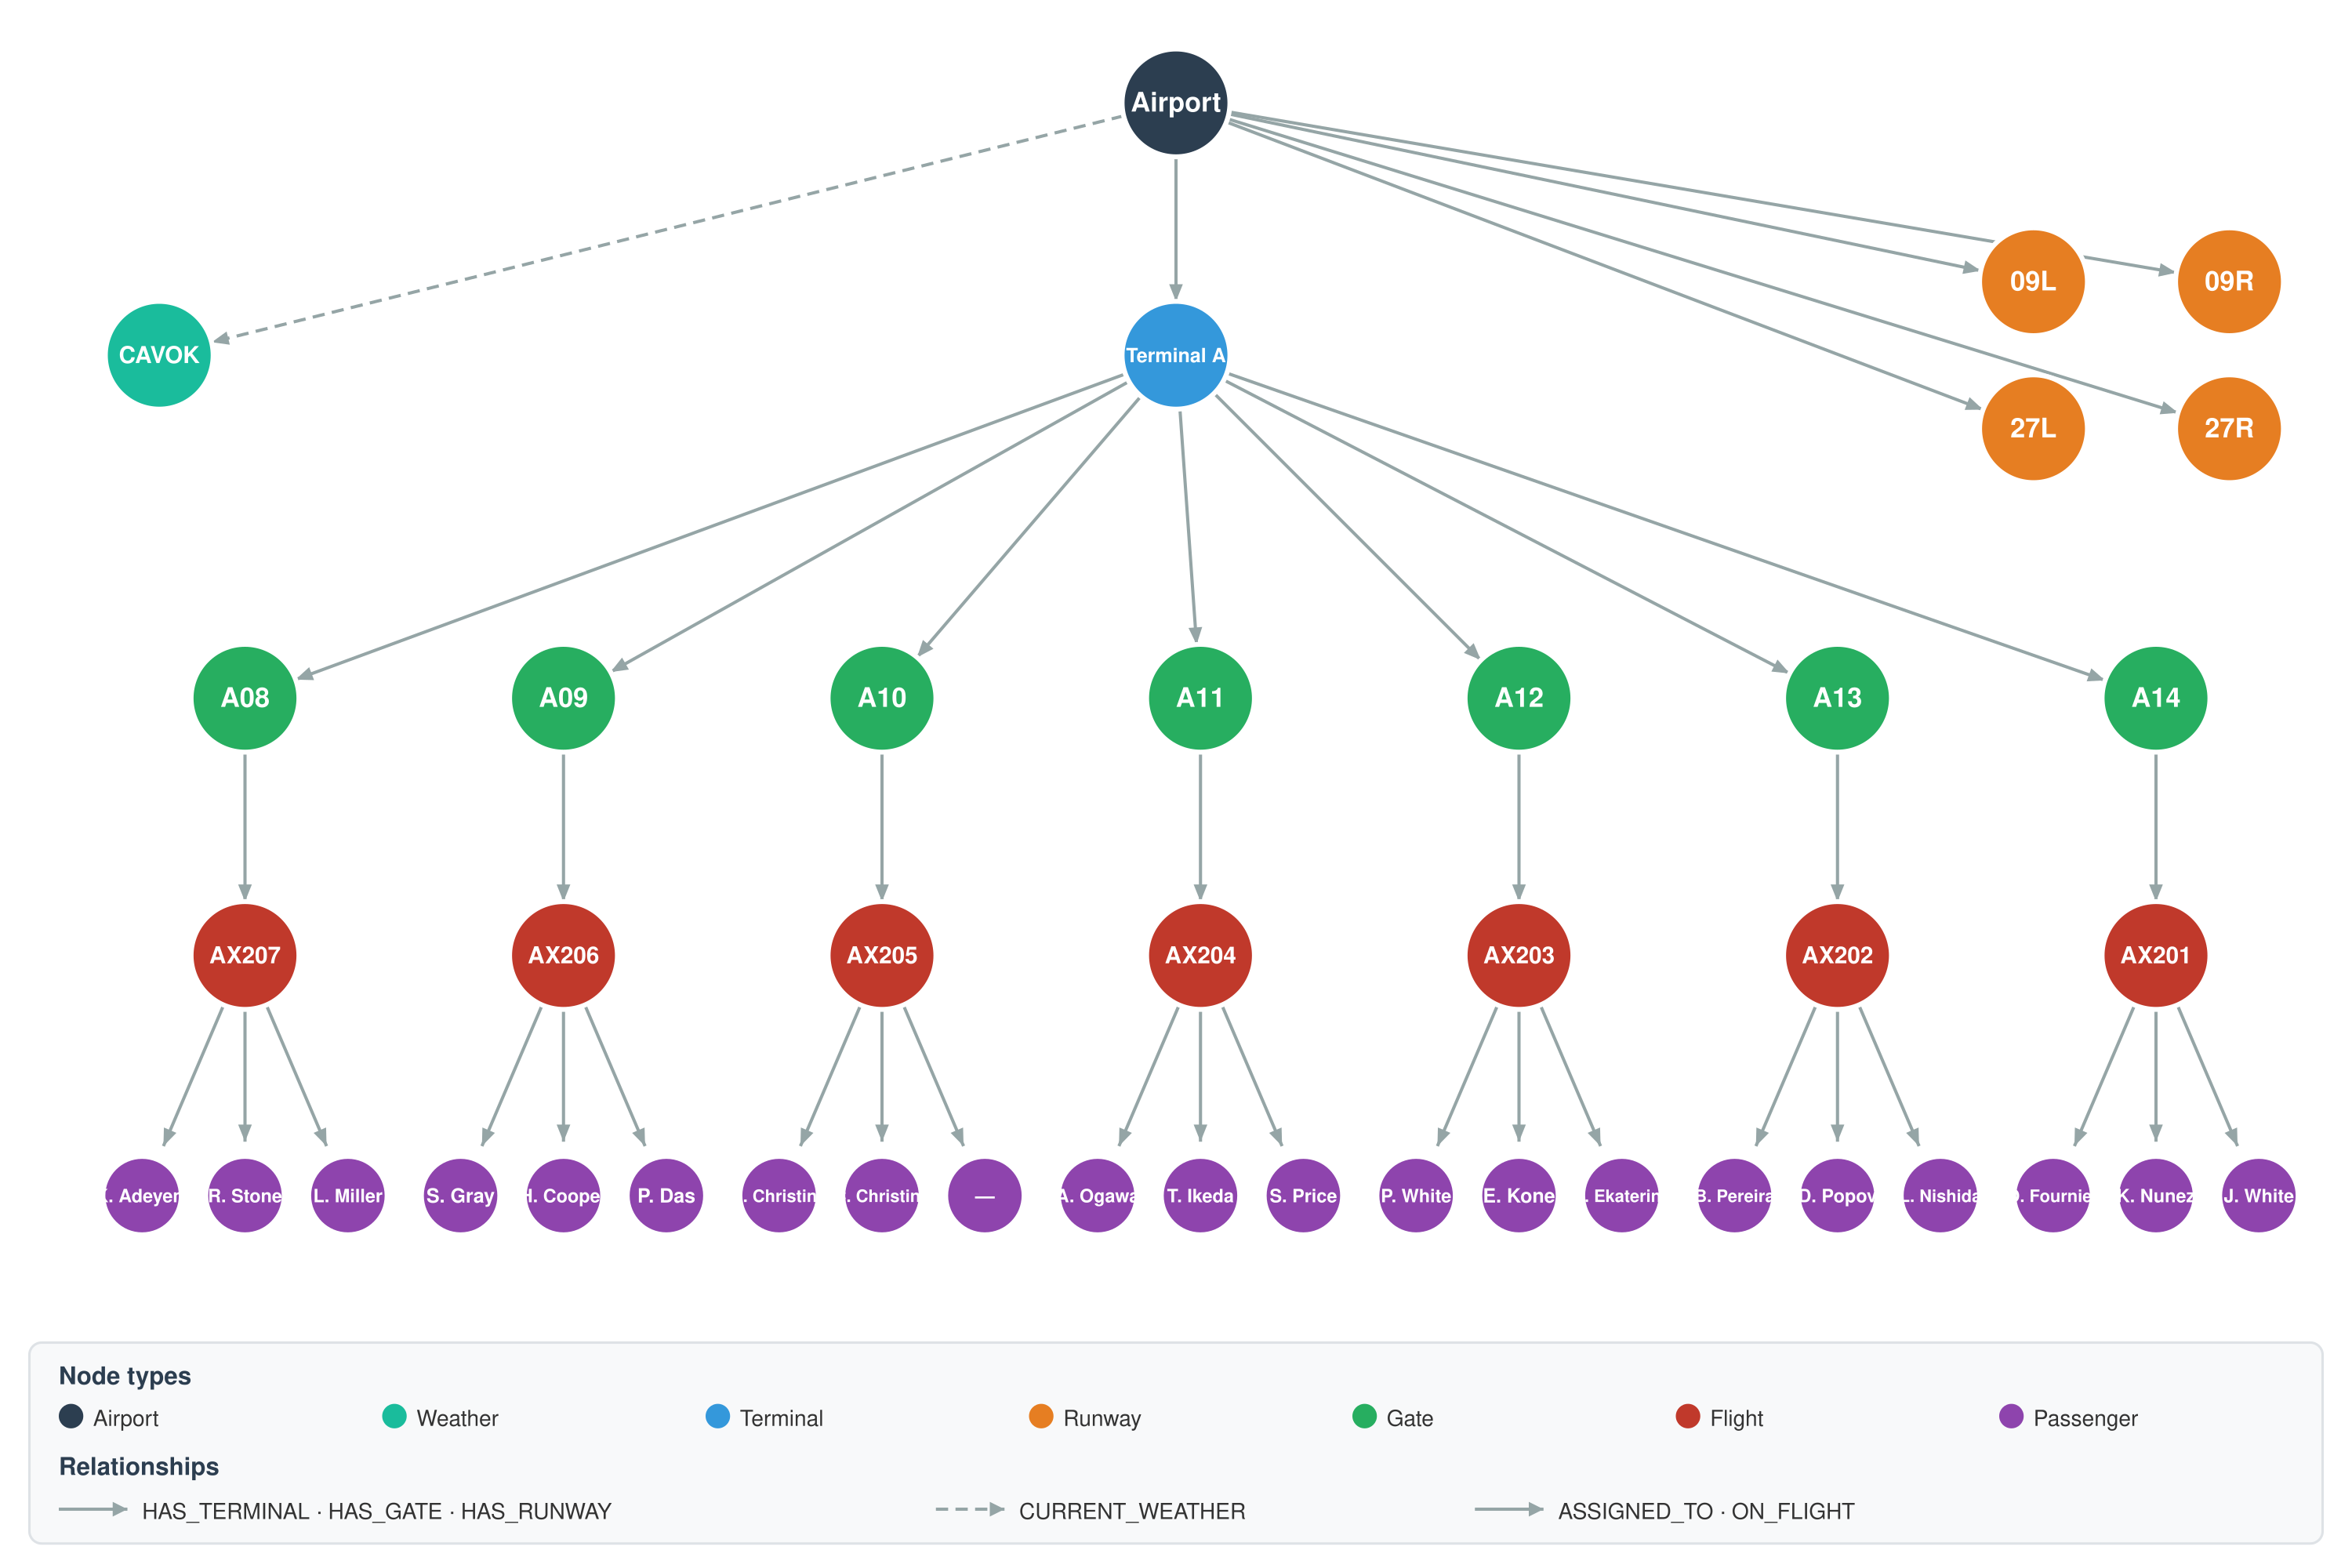
\includegraphics[width=1\linewidth]{figures/visualisation.png}
\caption{L0: Neo4j as source of truth and context broker.}
\label{fig:neo4j}
\end{figure}

\begin{figure}
\centering
\includegraphics[width=1\linewidth]{figures/data_sources.png}
\caption{L2: the shared data-source registry, exposing a single adapter interface to simulated, historical, and live providers alike. Each adapter normalises its source-specific input --- ADS-B flight positions, METAR/TAF weather, BTS schedule data, OurAirports/OpenFlights reference data --- into the same domain events consumed downstream, so a new data source can be added or swapped per theme without any change to the services, graph model, dashboards, or analytical code that consume it. This is the mechanism behind the twin's practical Open/Closed property described in Section~\ref{sec:implementation}.}
\label{fig:datasources}
\end{figure}

\begin{figure}
\centering
\includegraphics[width=1\linewidth]{figures/cost.png}
\caption{L3: the cost dashboard, the first decisional-layer capability, built entirely by consuming events emitted by the layers below rather than by any direct access to their internal state. It aggregates operational and disruption cost --- fuel, handling, and EC~261/2004 passenger-rights compensation --- into the profit-and-loss view maintained by the financial service, closing the causal chain traced in Section~\ref{sec:evaluation} from a weather-driven runway-capacity drop through to its quantified financial exposure.}
\label{fig:cost}
\end{figure}

These screenshots show what each layer looks like once built, not what happened underneath as it was added, so we checked the commit history directly. Five of the largest refactor and feature commits (\texttt{23bea42}, \texttt{8536eab}, \texttt{10536f1}, \texttt{4d8e4b4}, \texttt{22c5c18}) each modified between 41 and 94 files across four or more services at once. Two of these, \texttt{23bea42} and \texttt{22c5c18}, also changed L0's event-bus and graph-model documentation, so we inspected both line by line.

The clearest example is the introduction of the cost service in \texttt{22c5c18}. Adding it meant extending the event bus with a new topic, \texttt{cost.events}, and a new event type, \texttt{CostRecorded}; extending the graph model with a new node type, \texttt{CostRecord}, its relationships, and its indexes; and widening the consumer list of four existing topics (\texttt{flights.events}, \texttt{passengers.events}, \texttt{baggage.events}, \texttt{incidents.events}) so the new service could read them. None of this changed what an existing event carried or how an existing consumer parsed it. The same pattern holds in \texttt{23bea42}, which added command topics for flights, passengers, and baggage alongside new event types, again without reshaping anything that already existed. Where existing dispatch code was touched, for instance cost-service's handler being extracted into a shared \texttt{process_envelope} function with added idempotency tracking, the same event cases and topic subscriptions were retained throughout.

This is what we mean by progressive fidelity in practice. Adding a new service, and even refactoring code around it, is expected as the system grows; what matters is whether the core contracts underneath stay intact. Across the commits audited here, the skills and event contracts a service already depended on stayed the same. We extended capability, we did not rewrite what was already working.

\subsection{Specification and skill file density}

The repository contains 90 commits on \texttt{main}, ten service directories (nine domain services + the API gateway) comprising 109 files, nine per-service specification files (\texttt{SPEC.md}), seven cross-cutting skill files, eight architecture documents, and two agent-facing entry points (\texttt{AGENTS.md}, \texttt{CLAUDE.md}). This density supports the specification-first discipline argued for in Section~\ref{sec:methodology}: the two commits examined above that extended the event contract also updated the corresponding architecture documents in the same commit, \texttt{EVENT_BUS.md} in both cases and \texttt{DATA_MODEL.md} and \texttt{docs/services/cost-service/SPEC.md} in \texttt{22c5c18}, rather than leaving code and specification to drift apart.

A mid-project audit also found cases where documentation and running code had drifted, discussed alongside its remediation in Section~\ref{sec:discussion}.

\section{Discussion and Conclusion}\label{sec:discussion}

The results address the two research questions directly. \textbf{RQ1} asked whether fidelity can be increased while preserving previously implemented layers. EVSK provides evidence that it can: new capabilities were added by extending existing contracts rather than restructuring lower layers. Configuration-driven airport identity, shared Kafka infrastructure, and hexagonal boundaries helped keep these interfaces stable as the system grew. The key result is therefore not the number of layers itself, but the use of explicit contracts to make fidelity an evolutionary property of the architecture.

\textbf{RQ2} asked whether specification-first development can preserve these contracts during sustained implementation, and where it requires independent verification. The experience was positive but not sufficient on its own. A mid-project audit found boundary failures including diverging duplicated constants, recommendations that were not connected to command topics, and an ML endpoint that reported success without having trained a model. These failures show that specifications constrain intended behaviour but do not guarantee implementation conformance. Periodic audits and mutation-style guards~\cite{demillo1978} were therefore necessary complements.

The two findings are complementary: \emph{the architecture defines what must remain stable; the methodology helps developers preserve it}. Neither is sufficient alone. A layered architecture can drift without verification, while a detailed specification can faithfully encode an incorrect boundary. The practical lesson from EVSK is that explicit contracts, specifications, and systematic verification should be treated as a single development discipline.

The approach is not specific to airports. Other cyber-physical domains with progressively increasing fidelity, such as ports, hospitals, and warehouses, could use the same pattern. However, this study is a single-case investigation with a small team, one domain, and synthetic ground truth~\cite{runeson2009}. Learning effects are also confounded with the effects of specification-first development and of the AI assistance used during implementation, so the observed productivity and defect trends should not be assumed to generalise.

Future work includes completing command-topic coverage for decisional capabilities, using EVSK's deterministic event history as a benchmark for multi-agent reinforcement learning, and extending the configuration-driven architecture to federated multi-airport studies.

Overall, EVSK supports \textbf{RQ1} by demonstrating the feasibility of contract-preserving progressive fidelity, and supports \textbf{RQ2} by showing that specification-first development can help maintain those contracts during sustained implementation, while requiring independent verification. The broader contribution is an architectural and development pattern for growing complex digital twins without making each increase in fidelity a reason to rebuild the layers beneath it.

\section\*{Acknowledgments and Use of AI}
This research received no specific grant from any funding agency in the public, commercial, or not-for-profit sectors. All computation, development, and infrastructure for the EVSK implementation were carried out on the authors' own resources, without external infrastructure support. The authors thank colleagues at the Luxembourg Institute of Science and Technology for their review of and feedback on earlier drafts of this manuscript.

Artificial intelligence tools were used to support the writing and editing of this manuscript, including text rephrasing, proofreading, and improving clarity. All scientific content, interpretations, and conclusions were produced and validated by the authors, who take full responsibility for the accuracy and integrity of all statements in the paper.

\newpage
\section\*{Annex}

\begin{figure}[H]
\centering
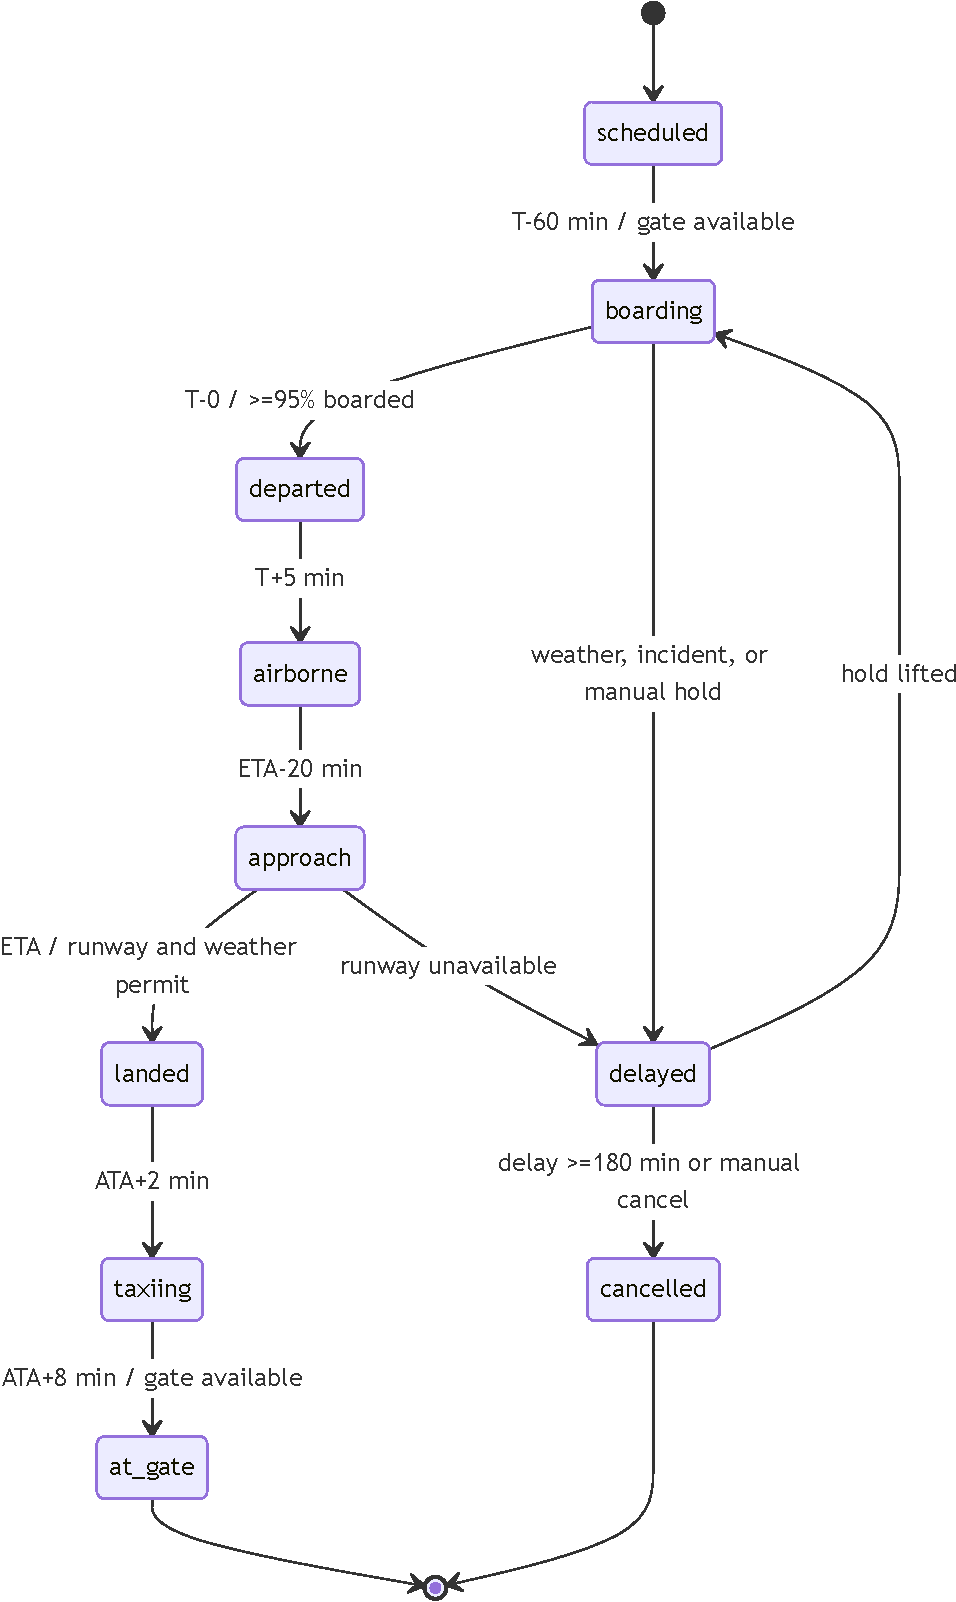
\includegraphics[width=\textwidth]{figures/flight-lifecycle.pdf}
\caption{Flight lifecycle driven by simulated time and constrained by gates, runways, weather, incidents, and boarding progress.}
\label{fig:flight-lifecycle}
\end{figure}

\begin{figure}[H]
\centering
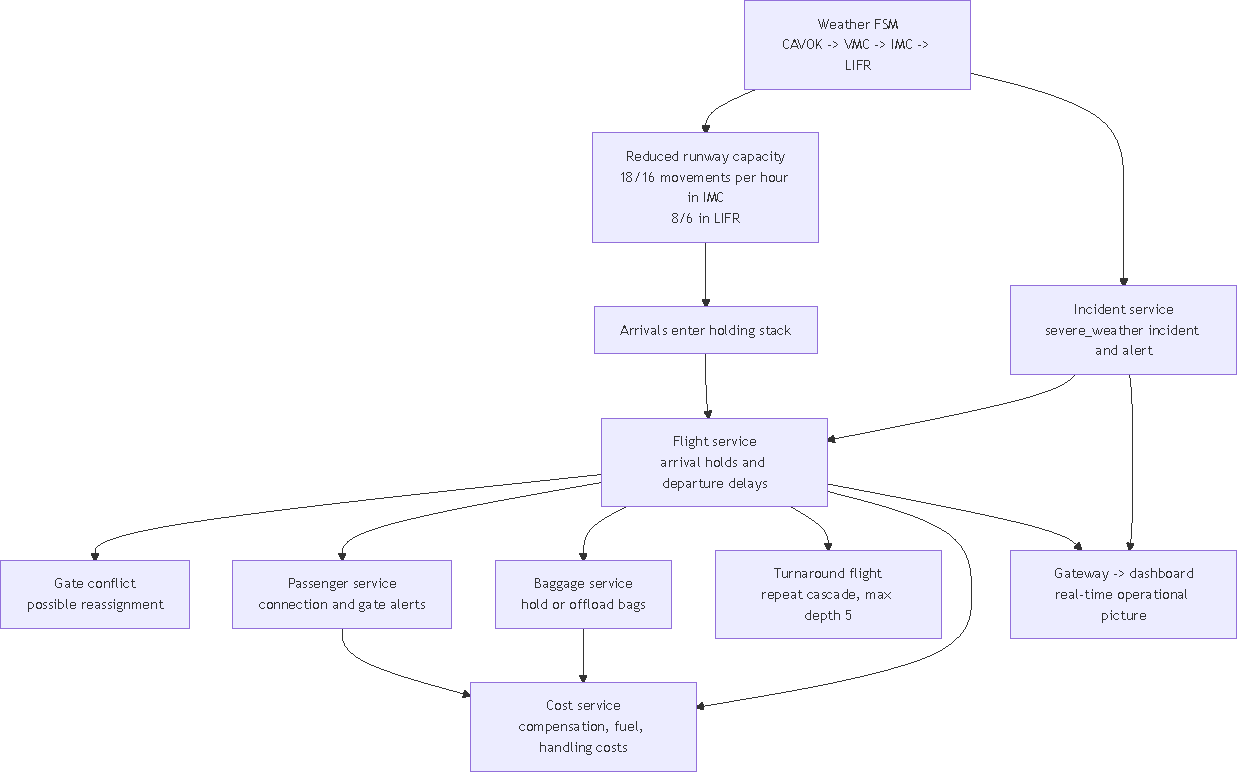
\includegraphics[width=\textwidth]{figures/weather-cascade.pdf}
\caption{Causal propagation from weather degradation to runway capacity, flight delays, passenger and baggage disruption, and operational cost.}
\label{fig:weather-cascade}
\end{figure}

\begin{figure}[H]
\centering
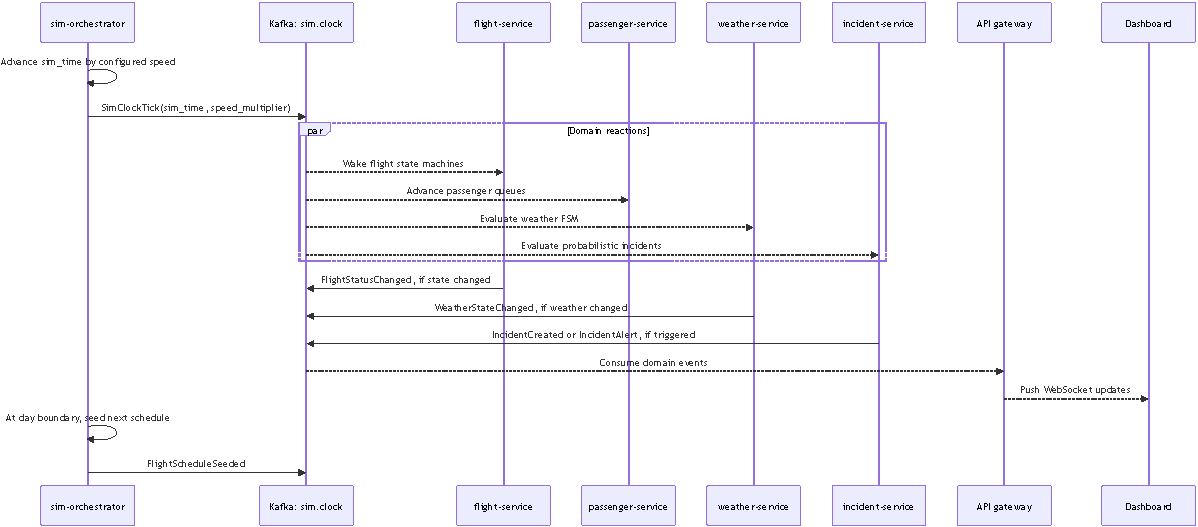
\includegraphics[width=\textwidth]{figures/clock.pdf}
\caption{Simulation-clock coordination in EVSK. A single virtual-time stream drives every service, and resulting facts are pushed to the dashboard through the gateway.}
\label{fig:clock}
\end{figure}

\newpage
%
% ---- Bibliography ----
%
\bibliographystyle{splncs03_unsrt}
\bibliography{refs.bib}

\end{document}
